\section{Evaluation}
\label{lo:sec:results}

\newcommand\redcircle{%
\begin{tikzpicture}\draw[red] (0,0) circle (1mm);\end{tikzpicture}}

\subsection{Method}
We have evaluated our tool on a suite of benchmark examples that consists of
several applications that have recurring inter-iteration dependences:
\begin{itemize}

\item A simple loop, \verb|sum|, that sums the elements in an array.

\item Two kernels from Livermore Loops~\cite{livermore}: \verb|dotprod|, which
computes the dot product of two vectors, and \verb|tridiag|, which solves a
tridiagonal linear system of equations.

\item Nine kernels from PolyBench~\cite{polybench}, which calculate
matrix/vector transpositions, additions and multiplications (\verb|2mm|,
\verb|3mm|, \verb|atax|, \verb|gemm|, \verb|gemver|, \verb|mvt|), the
bi-conjugate gradient stabilized method (\verb|bicg|), the Seidel stencil
computation (\verb|seidel|), and symmetric rank-2k operations
(\verb|syr2k|).

\end{itemize}

All elements of input arrays and matrices are set to be single-precision
floating-point values bounded by 0 and 1.  We optimized all of these benchmark
examples using our tool, specifically targeting the Xilinx Virtex7 device
running at 333~MHz, for the three objectives of accuracy, resource utilization
and latency simultaneously.  We then used Vivado HLS 2015.2~\cite{vivado_hls}
to synthesize the resulting optimized programs into RTL implementations for
exact latency information, and performed place-and-route using Vivado Design
Suite 2015.2~\cite{vivado_ds}, to obtain exact resource utilization statistics.
Our tool produces a three-dimensional Pareto frontier for each program.

\subsection{Results}

\begin{table}[t]
    \centering
\scriptsize
    %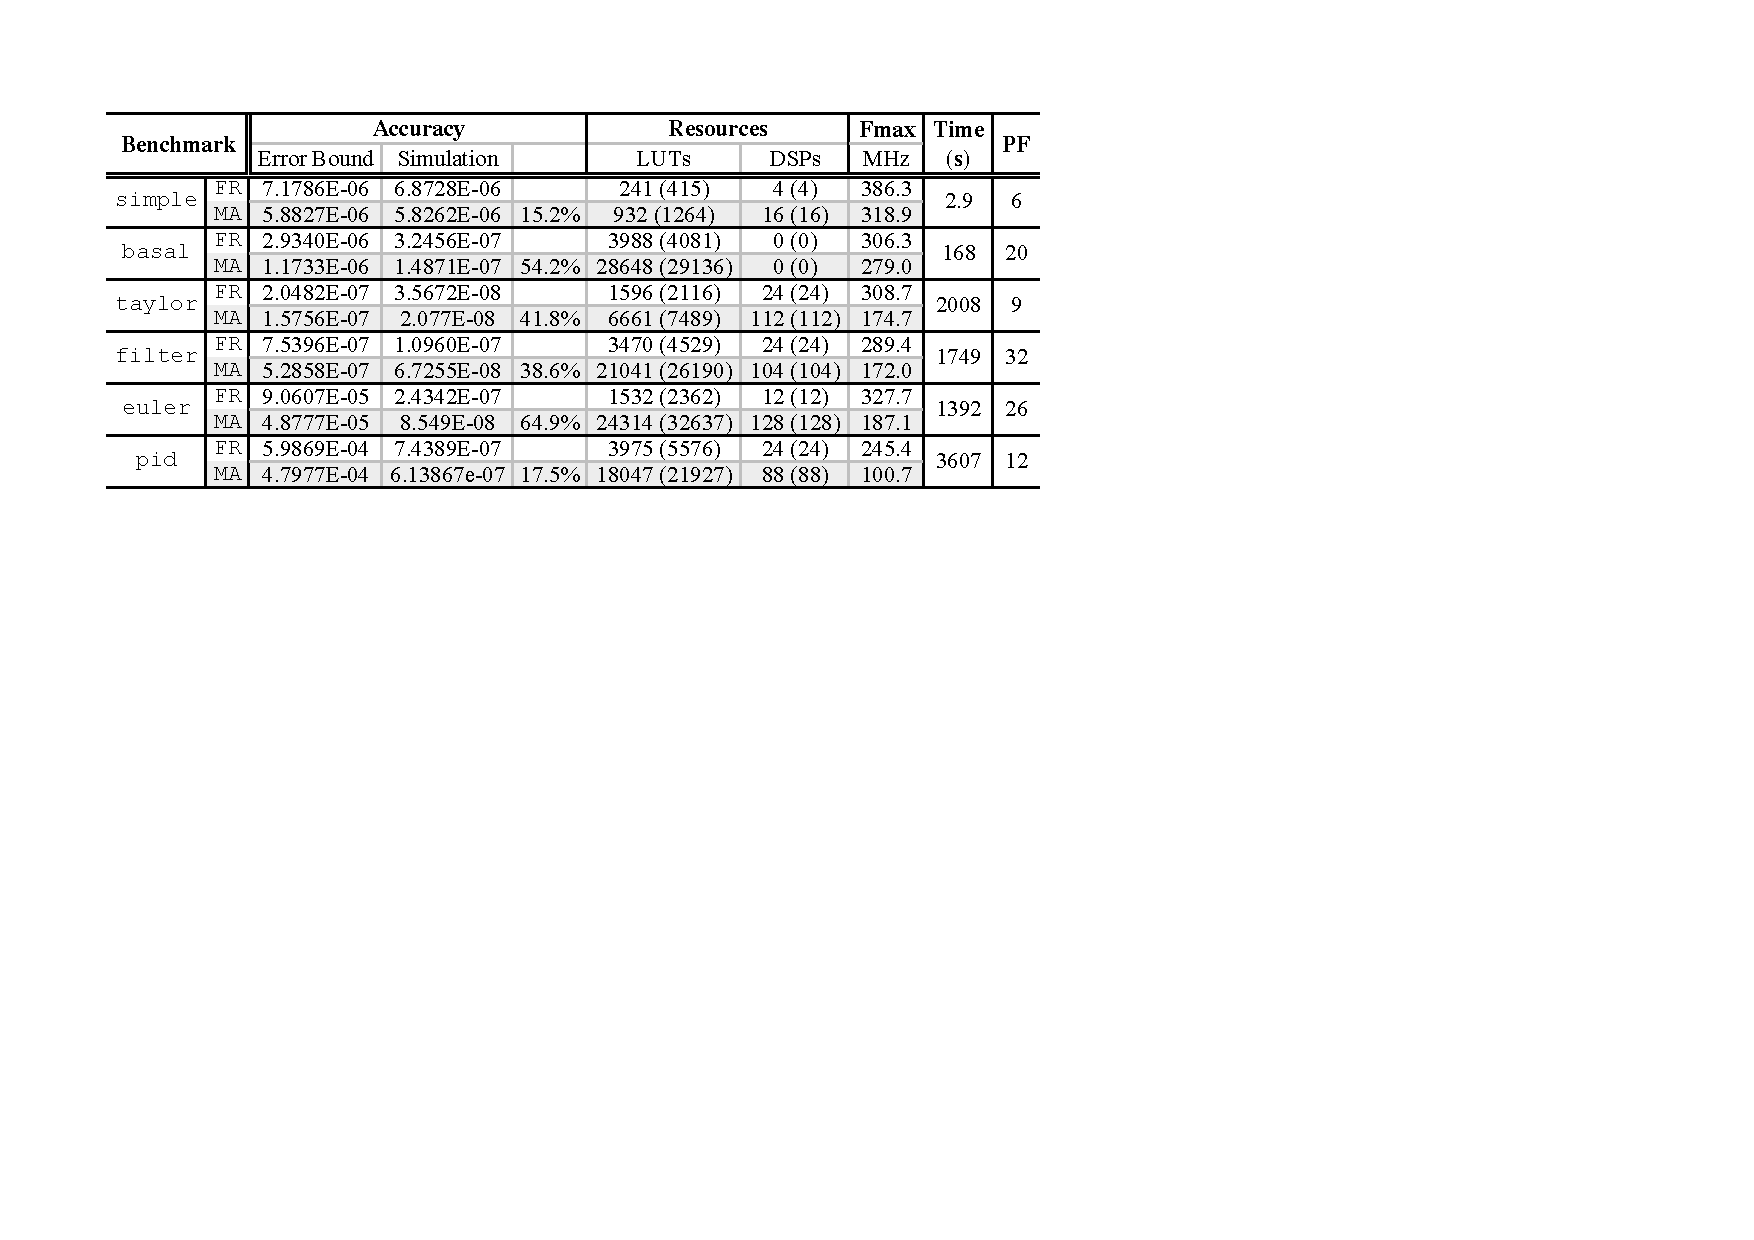
\includegraphics[width=\linewidth]{results}

\renewcommand\arraycolsep{0.45mm}
\newcommand\unitk{\,\text{k}}
\newcommand\unitm{\,\text{m}}
\newcommand\unitmu{\,\text{\textmu}}
\newcommand\unitM{\,\text{M}}
\newcommand\unitG{\,\text{G}}
\newcommand\Mid[1]{\multirow{2}*{$#1$}}
\newcommand\Shade{\cellcolor{black!10}}
\newcommand\name[1]{\texttt{\scriptsize #1}}
$\begin{array}{l|r|r|r|r|r|r|r|r|r}
\multicolumn{1}{c|}{\text{Name}} & \multicolumn{1}{c|}{\text{DSPs}} & \multicolumn{2}{c|}{\text{LUTs}} & \multicolumn{2}{c|}{\text{Error}} & \multicolumn{1}{c|}{\text{Clock}} & \multicolumn{3}{c}{\text{Latency}}
\\
& & & \multicolumn{1}{c|}{\text{ratio}} & &
\multicolumn{1}{c|}{\text{ratio}} & \multicolumn{1}{c|}{\text{(ns)}} & \multicolumn{1}{c|}{\text{(cycles)}} & \multicolumn{1}{c|}{\text{(s)}} &
\multicolumn{1}{c}{\text{ratio}}
\\ \hline
\Mid{\name{sum}} & 2 & 303 & \Mid{0.257} & 914\unitmu & \Mid{7.93} & 2.54 & 41.0\unitk
& 104\unitmu & \Mid{12.8} \\
& \Shade 4 & \Shade 1181 & & \Shade 1.15\unitmu & & \Shade 2.54 & \Shade 3.21\unitk & \Shade 8.17\unitmu &
\\ \hline
\Mid{\name{dotprod}} & 5 & 411 & \Mid{0.231} & 926\unitmu & \Mid{7.29} & 2.54 &
41.0\unitk & 104\unitmu & \Mid{12.4} \\
& \Shade 10 & \Shade 1781 & & \Shade 127\unitmu & & \Shade 2.62 & \Shade
3.23\unitk & \Shade 8.44\unitmu &
\\ \hline
\Mid{\name{tridiag}} & 5 & 470 & \Mid{0.288} & 63.1\unitmu & \Mid{1.06} & 2.54 &
17.8\unitM & 45.3\unitm & \Mid{3.41} \\
& \Shade 8 & \Shade 1631 & & \Shade 59.4\unitmu & & \Shade 2.69 & \Shade 4.93\unitM & \Shade 13.3\unitm &
\\ \hline
\Mid{\name{2mm}} & 5 & 781 & \Mid{0.385} & 209 & \Mid{3.40} & 2.79 & 20.4\unitG & 57.0
& \Mid{7.46} \\
& \Shade 8 & \Shade 2029 & & \Shade 61.4 & & \Shade 2.92 & \Shade 2.62\unitG & \Shade 7.64 &
\\ \hline
\Mid{\name{3mm}} & 5 & 760 & \Mid{0.207} & 114 & \Mid{6.76} & 2.55 & 32.3\unitG & 82.3 &
\Mid{9.13} \\
& \Shade 10 & \Shade 3677 & & \Shade 16.9 & & \Shade 2.82 & \Shade 3.19\unitG & \Shade 9.01 &
\\ \hline
\Mid{\name{atax}} & 5 & 627 & \Mid{0.507} & 353\unitm & \Mid{1.54} & 2.60 & 176\unitM
& 457\unitm & \Mid{5.42} \\
& \Shade 5 & \Shade 1237 & & \Shade 230\unitm & & \Shade 2.61 & \Shade
32.4\unitM & \Shade 84.3\unitm &
\\ \hline
\Mid{\name{bicg}} & 5 & 427 & \Mid{0.304} & 887\unitmu & \Mid{6.72} & 2.54 & 160\unitM &
407\unitm & \Mid{8.98} \\
& \Shade 5 & \Shade 1406 & & \Shade 132\unitmu & & \Shade 2.78 & \Shade 16.3\unitM & \Shade 45.3\unitm &
\\ \hline
\Mid{\name{gemm}} & 5 & 524 & \Mid{0.234} & 1.99 & \Mid{2.97} & 2.54 & 10.8\unitG &
27.4 & \Mid{9.13} \\
& \Shade 10 & \Shade 2240 & & \Shade 0.67 & & \Shade 2.69 & \Shade 1.12\unitG & \Shade 3.00 &
\\ \hline
\Mid{\name{seidel}} & 5 & 620 & \Mid{0.349} & 10.7\unitmu & \Mid{2.46} & 2.60 & {960}\unitM
& 2.50 & \Mid{7.16} \\
& \Shade 8 & \Shade 1778 & & \Shade 4.31\unitmu & & \Shade 2.66 & \Shade {131}\unitM & \Shade 0.349 & \\ \hline
\Mid{\name{gemver}} & 5 & 809 & \Mid{0.382} & 7.28\unitM & \Mid{4.46} & 2.87 &
{23.1}\unitM & 66.2\unitm & 3.15 \\
& \Shade 5 & \Shade 2120 & & \Shade 1.63\unitM & & \Shade 2.77 & \Shade {7.60}\unitM & \Shade 2.10\unitm & (8.29)
\\ \hline
\Mid{\name{mvt}} & 5 & 701 & \Mid{0.251} & 91.0\unitmu & \Mid{3.32} & 2.56 & {23.1}\unitM &
59.1\unitm & 7.49 \\
& \Shade 10 & \Shade 2793 & & \Shade 27.4\unitmu & & \Shade 2.80 & \Shade {2.82}\unitM & \Shade 7.89\unitm & (9.30)
\\ \hline
\Mid{\name{syr2k}} & 5 & 709 & \Mid{0.259} & 250\unitmu & \Mid{4.07} & 2.89 & {14.0}\unitG &
40.3 & 6.95 \\
& \Shade 10 & \Shade 2740 & & \Shade 61.4\unitmu & & \Shade 2.71 & \Shade {2.14}\unitG & \Shade 5.80 & (7.62)
\\ \hline
\multicolumn{3}{r|}{\Mid{\text{Geomean}}} & \Mid{0.289} & & \Mid{3.69} & \multicolumn{3}{r|}{} & 7.19 \\
\multicolumn{3}{r|}{} & & & & \multicolumn{3}{r|}{} & (8.01)
\\ \hline
\end{array}$
    \caption{%
        Comparisons of the original (non-shaded rows) and the optimized program
        with lowest latency (shaded rows), for each benchmark. Values in
        parentheses are obtained after slightly tweaking our experimental
        set-up; see Section~\ref{lo:sec:results_discussion}.  We performed
        place-and-route for exact statistics.
    }\label{lo:tab:results}
\end{table}

Table~\ref{lo:tab:results} compares, for each benchmark in our evaluation
set, the performance metrics of the original program against those of the
program with the smallest latency discovered by our tool. We synthesized
each program to a circuit to obtain exact statistics, which are shown in
Table~\ref{lo:tab:results}.


\begin{figure}[ht]
    \centering
    \begin{tikzpicture}
        \begin{axis}[
                ylabel={\small Estimated}, xlabel={\small Actual},
                height=100mm, width=100mm, ylabel near ticks,
                scaled ticks=base 10:-3,
                ymax=4000, xmax=4000, ymin=0, xmin=0]
            \pgfplotstableread[col sep = comma]{latopt/csv/lut.csv}\lutcsv
            \addplot[draw=none, mark=*, draw opacity=0, fill opacity=0.5]
                table [y=Estimate, x=Actual] \lutcsv;
            \addplot[mark=none, draw=none]
                table
                [x=Actual, y={create col/linear regression={y=Estimate}}]
                \lutcsv;
            \xdef\slope{\pgfplotstableregressiona} % save the slope parameter
            \xdef\intercept{\pgfplotstableregressionb} % save the intercept parameter
            \addplot [no markers, domain=0:4000] {\intercept+\slope*x};
        \end{axis}
    \end{tikzpicture}
    \caption{%
        Comparisons of our estimated LUT counts against actual LUT counts from
        Vivado HLS\@.}
    \label{lo:fig:lut}
\end{figure}

\begin{figure}[ht]
    \centering
    \begin{tikzpicture}
        \begin{loglogaxis}[
                ylabel={\small Estimated}, xlabel={\small Actual},
                height=100mm, width=100mm, ylabel near ticks,
                %scaled ticks=base 10:-9,
                xmin=1000, ymin=1000, xmax=100000000000, ymax=100000000000]
            \pgfplotstableread[col sep = comma]{latopt/csv/lat.csv}\latcsv
            \addplot[draw=none, mark=*, draw opacity=0, fill opacity=0.5]
                table [y=Estimate, x=Actual] \latcsv;
            \addplot[mark=none, draw=none]
                table
                [x=Actual, y={create col/linear regression={y=Estimate}}]
                \latcsv;
            \xdef\slope{\pgfplotstableregressiona} % save the slope parameter
            \xdef\intercept{\pgfplotstableregressionb} % save the intercept parameter
            \addplot
                [no markers, domain=1000:100000000000] {\intercept+\slope*x};
        \end{loglogaxis}
    \end{tikzpicture}
    \caption{%
        Comparisons of our estimated latency statistics against actual latency
        from Vivado HLS\@.}
    \label{lo:fig:lat}
\end{figure}

\begin{figure*}[t]
    \centering
    \tikzset{%
        every axis/.style={%
            height=70mm, width=70mm, ylabel near ticks, try min ticks=5},
        every plot/.style={draw=none},
        normal points/.style={mark=*, draw opacity=0, fill opacity=0.5},
        origin point/.style={mark=x, mark size=3},
        special point/.style={mark=o, color=red, mark size=3},
    }
    \pgfplotstableread[col sep=comma, row sep=newline]
        {latopt/csv/seidel.csv}\seidel

    \begin{tikzpicture}
        \begin{axis}[
                ylabel={\small LUT count},
                xlabel={\small Latency (cycles)},
                scaled y ticks=base 10:-3,
            ]
            \addplot[normal points, select coords between index={1}{24}]
                table [y=lut, x=latency]\seidel;
            \addplot[normal points,  select coords between index={26}{28}]
                table [y=lut, x=latency]\seidel;
            \addplot[origin point, select coords between index={0}{0}]
                table [y=lut, x=latency]\seidel;
            \addplot[special point, select coords between index={25}{25}]
                table [y=lut, x=latency]\seidel;
        \end{axis}
    \end{tikzpicture}

    \begin{tikzpicture}
        \begin{axis}[
                ylabel={\small LUT count},
                xlabel={\small Error},
                scaled y ticks=base 10:-3,
            ]
            \addplot[normal points, select coords between index={1}{24}]
                table [y=lut, x=error]\seidel;
            \addplot[normal points,  select coords between index={26}{28}]
                table [y=lut, x=error]\seidel;
            \addplot[origin point, select coords between index={0}{0}]
                table [y=lut, x=error]\seidel;
            \addplot[special point, select coords between index={25}{25}]
                table [y=lut, x=error]\seidel;
        \end{axis}
    \end{tikzpicture}

    \begin{tikzpicture}
        \begin{axis}[
                ylabel={\small Latency (cycles)},
                xlabel={\small Error},
            ]
            \addplot[normal points, select coords between index={1}{24}]
                table [y=latency, x=error]\seidel;
            \addplot[normal points, select coords between index={26}{28}]
                table [y=latency, x=error]\seidel;
            \addplot[origin point, select coords between index={0}{0}]
                table [y=latency, x=error]\seidel;
            \addplot[special point, select coords between index={25}{25}]
                table [y=latency, x=error]\seidel;
        \end{axis}
    \end{tikzpicture}
    \caption{%
        Pareto-optimal variants of the Seidel stencil program from
        Figure~\ref{lo:fig:seidel_prog}. Each graph shows a 2D projection
        of the 3D Pareto frontier. In each graph, the original program is
        marked $\times$, and the lowest-latency variant obtained by arithmetic
        transformations alone is marked \protect\redcircle.}
    \label{lo:fig:seidel}
\end{figure*}

Figure~\ref{lo:fig:lut} compares our estimated LUT counts (vertical axis)
against the exact LUT counts (horizontal axis) obtained by synthesizing RTL
implementations of each program in Table~\ref{lo:tab:results}.  Although our
estimates deviate from the exact values, because we compute lower bounds on
resource utilizations, and finite state machines synthesized and address
calculation are not taken into account, our estimate can still accurately
predict the general trend---a linear regression of all scatter points finds
$R^2 = 0.9344$.

Figure~\ref{lo:fig:lat} compares our latency estimates (vertical axis)
against the actual latency values (horizontal axis). The solid line
represents the linear regression of data points that we have gathered in
Table~\ref{lo:tab:results}. This line is a tight fit with our data, with $R^2 =
0.9959$, which indicates that our latency estimation can accurately predict the
exact latency of synthesized implementations.

Returning to our motivating example from Section~\ref{lo:sec:motivation},
Figure~\ref{lo:fig:seidel} demonstrates the range of optimized programs
discovered by our tool when applied to the Seidel stencil loop kernel. In
the figure, $\times$-points indicate the original program. By using only the
rules of real arithmetic, our tool finds a more efficient program that can
improve run time by 2.5$\times$, as shown by the \redcircle-points. However,
by enabling partial loop unrolling and our dependence elimination rules, the
performance is further improved, resulting in a 6.7$\times$ reduction of
total run time.  Furthermore, we have found that numerical accuracy can often
be optimized at the same time as we optimize the initiation intervals of
loops. Because by partially unrolling loops, the sizes of the expressions in
loop grow, which provides our tool a greater freedom in terms of discovering
more accurate expressions. In this example, the most efficient program is
also the most accurate one: it minimizes round-off errors by approximately
2.5$\times$. It is worth noting that our tool can detect that as it explores
deep levels of partial loop unrolling, we start to see a diminishing return
in performance as it hits a bottleneck in memory bandwidth.  This is due to
the fact that Vivado HLS synthesizes dual port RAMs for arrays, and in one
clock cycle we can only read from the memory allocating array twice.  Our
optimization flow is aware of this bottleneck and stops exploring further loop
unrolling.

Similar graphs for the other benchmarks can be viewed
online,\footnote{\url{https://admk.github.io/soap/plot.html}} each showing
three projections from different axes of the 3D Pareto frontier. Our web page
can be used to interactively explore the positions of each data point on the
three projections simultaneously, and view the corresponding generated C
programs.

\subsection{Discussion}
\label{lo:sec:results_discussion}

As demonstrated by Figure~\ref{lo:fig:lat}, our tool generally produces
accurate latency estimates. However, we have discovered a few notable
discrepancies. For instance, \verb|gemver|, \verb|mvt| and \verb|syr2k| all
have significant differences between our estimated latency and the actual
latency from synthesized RTL implementations.  An inspection of these programs
reveals that they all share a common programming idiom:
%
\begin{lstlisting}
  for (int i=0; i<N; i++)
    for (int j=0; j<N; j++)
      x[i] += ...;
\end{lstlisting}
%
We found that Vivado HLS occasionally fails to find the optimal schedule,
predicted by our tool, that could pipeline this loop as tightly as possible.
By rewriting the above code into:
%
\begin{lstlisting}
  for (int i=0; i<N; i++) {
    float sum = x[i];
    for (int j=0; j<N; j++)
      sum += ...;
    x[i] += sum;
  }
\end{lstlisting}
%
We fix this problem, and enable Vivado HLS to generate a hardware
implementation with the expected $\II$. The ratios in parentheses in
Table~\ref{lo:tab:results} reflect the speedup by performing this simple fix.

%%% Local Variables:
%%% mode: latex
%%% TeX-master: "paper"
%%% End:
